% !TeX encoding = UTF-8
% !TeX spellcheck = en_US
\section{Case studies}

This section presents two case studies in simulation to demonstrate the design of linear and nonlinear MPCs. The objective here is to hopefully demonstrate how the package syntax facilitates the implementation and testing of predictive controllers and state estimators. The first example details how to apply a MPC on a plant at each discrete time step. The second uses higher-level functionalities to quickly simulate closed-loop systems. 

\subsection{Linear Design: Continously Stirred Tank Reactor}

\subsubsection{Linear Model}

The example considers a continuously stirred tank reactor (CSTR) with a cold and hot water intakes, fed at a respective flow rate of $u_c$ and $u_h$. The manipulated input vector is thus $\mathbf{u} = [\begin{smallmatrix}u_c & u_h\end{smallmatrix}]'$. The liquid level $y_L$ and temperature $y_T$ constitute the measured output vector $\mathbf{y} = [\begin{smallmatrix}y_L & y_T\end{smallmatrix}]'$. Fig. 1 depicts the instrumentation installed on the plant.

At the steady-state operating point $u_c=u_h=20$, $y_L=50$, and $y_T=30$, the following linear model accurately describes the plant dynamics:
\begin{equation}
\mathbf{G}(s) = \frac{\mathbf{y}(s)}{\mathbf{u}(s)} =
\begin{bmatrix}
    \frac{1.90}{18s+1} & \frac{1.90}{18s+1} \\[3pt]
    \frac{-0.74}{8s+1} & \frac{0.74}{8s+1}
\end{bmatrix}
\end{equation}
The syntax to construct a linear model with a sample time of $\SI{2}{\second}$ is:
\begin{minted}{julia}
using ModelPredictiveControl, ControlSystemsBase
G = [ tf(1.90, [18, 1]) tf(1.90, [18, 1]);
      tf(-0.74,[8, 1])  tf(0.74, [8, 1]) ]
model = setop!(LinModel(G, 2.0); uop=[20,20], yop=[50,30])
\end{minted}
\spacerepl
\begin{minted}{julia-repl}
Discrete-time linear model with a sample time Ts = 2.0 s and:
 2 manipulated inputs u
 2 states x
 2 outputs y
 0 measured disturbances d
\end{minted}
The \texttt{model} object will be used for two purposes : to construct our controller and as a plant simulator to test the design.

\subsubsection{Linear Model Predictive Controller}

The objective is to control both the water temperature and level while constraining the level above 45:
\begin{minted}{julia}
mpc = setconstraint!(LinMPC(model), ymin=[45, -Inf])
\end{minted}
\spacerepl
\begin{minted}{julia-repl}
LinMPC controller with a sample time Ts = 2.0 s, OSQP optimizer,
SteadyKalmanFilter estimator and:
 10 prediction steps Hp
  2 control steps Hc
  2 manipulated inputs u (0 integrating states)
  4 states x̂
  2 measured outputs ym (2 integrating states)
  0 unmeasured outputs yu
  0 measured disturbances d
\end{minted}
By default, \texttt{LinMPC} controllers use \texttt{OSQP.jl} \citep{osqp} to solve the problem, soft constraints on output predictions $\mathbf{\hat y}$ to ensure feasibility, and a \texttt{SteadyKalmanFilter} to estimate the plant states\footnote{As an alternative to state observers, we could have use an internal model structure with \texttt{estim = InternalModel(model)} and \texttt{mpc = setconstraint!(estim; nint\_u); ymin)}. It was tested on this example and it gives similar results.}. The default predictive and control horizons are \texttt{Hp=10+nk} and \texttt{Hc=2}, respectively, where \texttt{nk} is the number of delays in the linear model. An attentive reader will also notice that the Kalman filter estimates two additional states compared to the plant model. These are the integrating states for the unmeasured plant disturbances, and they are automatically added at the model output $\mathbf{y}$ by default if observability is preserved.

Before closing the loop, the actual plant inputs and measurements should initialize the estimates with \texttt{initstate!} to ensure a bumpless transfer. Since the plant is the linear model here, its output will initialize the states. \texttt{LinModel} objects are callable for this purpose. Once done, imposing step changes on the setpoint \texttt{ry} and on a load disturbance \texttt{ul} tests the closed-loop performance of \texttt{mpc}:
\begin{minted}{julia}
function test_mpc(mpc, plant)
    plant.x[:] .= 0; y = plant() # or evaloutput(plant)
    initstate!(mpc, plant.uop, y)
    N = 75; ry = [50, 30]; ul = 0
    U, Y, Ry = zeros(2, N), zeros(2, N), zeros(2, N)
    for i = 1:N
        i == 26 && (ry = [48, 35])
        i == 51 && (ul = -10)
        y = plant() # simulated measurements
        u = mpc(ry) # or moveinput!(mpc, ry)
        U[:,i], Y[:,i], Ry[:,i] = u, y, ry
        updatestate!(mpc, u, y) # update mpc estimate
        updatestate!(plant, u+[0,ul]) # update simulator
    end
    return U, Y, Ry
end
U_data, Y_data, Ry_data = test_mpc(mpc, model)
\end{minted}
Updating the internal states of \texttt{mpc} prepares the object for the \emph{next} time step. That is why the call is done at the end of the \texttt{for} loop. The same logic applies for \texttt{plant}. Lastly, we plot the closed-loop test with \texttt{Plots.jl}:
\begin{minted}{julia}
res = SimResult(mpc, U_data, Y_data; Ry_data)
using Plots; plot(res)
\end{minted}

\begin{figure}[h]
    \centering
    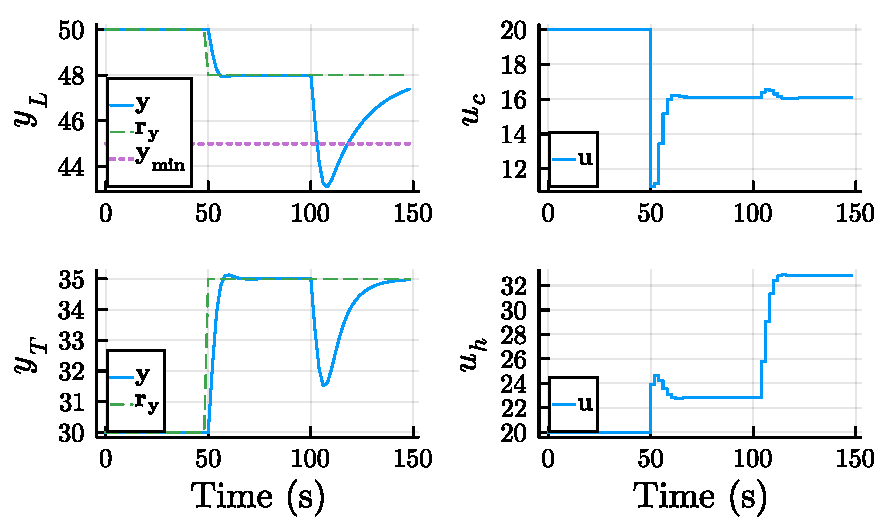
\includegraphics[width=\columnwidth]{fig/plot_LinMPC1.pdf}
    \caption{CSTR closed-loop simulation: $y_1=y_L$, $y_2=y_T$, $u_1=u_c$, and $u_2=u_h$.}
    \label{fig:plot_LinMPC1}
\end{figure}

\begin{figure}[h]
    \centering
    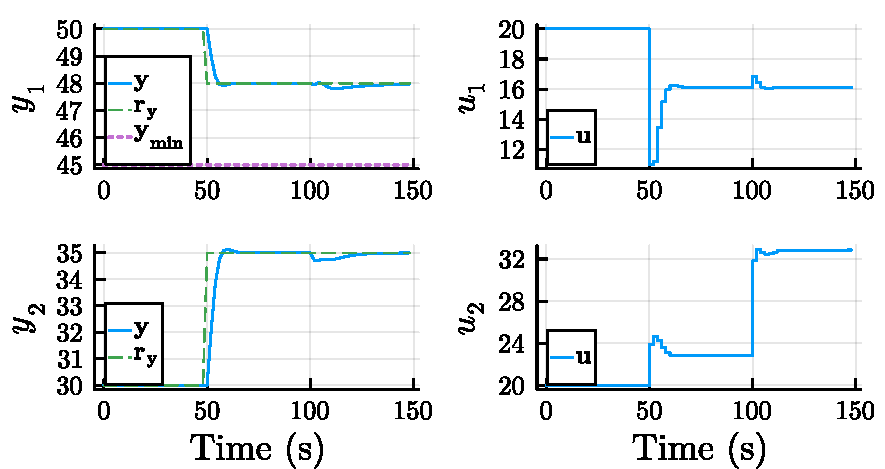
\includegraphics[width=\columnwidth]{fig/plot_LinMPC2.pdf}
    \caption{CSTR closed-loop simulation with feedforward: $y_1=y_L$, $y_2=y_T$, $u_1=u_c$, and $u_2=u_h$.}
    \label{fig:plot_LinMPC2}
\end{figure}

\cref{fig:plot_LinMPC1} shows that the controller violates the constraints around 110 s because of the disturbance. Adding feedforward compensation can mitigate this.

\subsubsection{Feedforward Compensation}

Suppose that the load disturbance $u_l$ of the last section is in fact caused by a separate hot water pipe that discharges into the tank. Measuring this flow rate allows us to incorporate feedforward compensation (FF) with the disturbance $\mathbf{d}=u_l$:

\begin{minted}{julia}
model_ff = LinModel([G G[1:2, 2]], 2.0; i_d=[3])
model_ff = setop!(model_ff; uop=[20,20], yop=[50,30], dop=[20])
\end{minted}
\spacerepl
\begin{minted}{julia-repl}
Discrete-time linear model with a sample time Ts = 2.0 s and:
 2 manipulated inputs u
 4 states x
 2 outputs y
 1 measured disturbances d
\end{minted}
The simulation needs a new \texttt{LinMPC} object based on \texttt{model\_ff} and a new test function that explicitly employs the current disturbance measurement:
\begin{minted}{julia}
mpc_ff = setconstraint!(LinMPC(model_ff), ymin=[45, -Inf])
function test_mpc_ff(mpc_ff, plant)
    plant.x[:] .= 0; y = plant(); d = [20]
    initstate!(mpc_ff, plant.uop, y, d)
    N = 75; ry = [50, 30]; ul = 0
    U, Y, Ry = zeros(2, N), zeros(2, N), zeros(2, N)
    for i = 1:N
        i == 26 && (ry = [48, 35])
        i == 51 && (ul = -10)
        y, d = plant(), [20+ul] # simulated measurements
        u = mpc_ff(ry, d) # d in arguments
        U[:,i], Y[:,i], Ry[:,i] = u, y, ry
        updatestate!(mpc_ff, u, y, d) # d in arguments
        updatestate!(plant, u+[0,ul])
    end
    return U, Y, Ry
end
U_data, Y_data, Ry_data = test_mpc_ff(mpc_ff, model)
res = SimResult(mpc, U_data, Y_data; Ry_data)
plot(res)
\end{minted}

\cref{fig:plot_LinMPC2} shows that the feedforward compensation handles the disturbance without violating the constraint.

\subsection{Nonlinear Design : Inverted Pendulum}
\label{sec.nonlinear_design}

\subsubsection{Nonlinear Model}

For this case study, the goal is to control the angular position $\theta$ of a pendulum attached to a motor, thus $\mathbf{y} = \theta$. The manipulated input is the motor torque $\mathbf{u} = \tau$. Fig. 4 depicts the instrumentation. The plant model is:
\begin{subequations}
\begin{align}
\dot{\theta}(t) &= \omega(t) \\
\dot{\omega}(t) &= -\frac{g}{L}\sin\big(\theta(t)\big) -\frac{K}{m}\omega(t) + \frac{1}{m L^2}\tau(t) \label{eq.pendulum_speed}
\end{align}
\end{subequations}
in which $g$ is the gravitational acceleration in \si{\meter\per\second\squared}, $L$, the pendulum length in \si{\meter}, $K$, the friction coefficient at the pivot point in \si{\kilogram\per\second}, and $m$, the mass attached at the end of the pendulum in \si{\kilogram}. Here, the explicit Euler method discretizes the system to construct a \texttt{NonLinModel}:
\begin{minted}{julia}
using ModelPredictiveControl
function pendulum(par, x, u)
    g, L, K, m = par     # [m/s²], [m], [kg/s], [kg]
    θ, ω = x[1], x[2]    # [rad], [rad/s]
    τ = u[1]             # [N m]
    return [ω, -g/L*sin(θ) - K/m*ω + τ/m/L^2]
end
par = (9.8, 0.4, 1.2, 0.3); Ts = 0.1
f(x, u, _ ) = x + Ts*pendulum(par, x, u) # Euler method
h(x, _ )    = [180/π*x[1]]  # [°]
nu, nx, ny = 1, 2, 1
model = NonLinModel(f, h, Ts, nu, nx, ny)
\end{minted}
\spacerepl
\begin{minted}{julia-repl}
Discrete-time nonlinear model with a sample time Ts = 0.1 s and:
 1 manipulated inputs u
 2 states x
 1 outputs y
 0 measured disturbances d
\end{minted}
The output function $\mathbf{h}$ converts the $\theta$ angle to degrees.

\subsubsection{Nonlinear State Estimator}

The state estimates produced by an \texttt{UnscentedKalmanFilter} will feed the controller:

\begin{minted}{julia}
σQ = [0.1, 0.5]; σR=[0.5]; nint_u=[1]; σQint_u=[0.1]
estim = UnscentedKalmanFilter(model; σQ, σR, nint_u, σQint_u)
\end{minted}
\spacerepl
\begin{minted}{julia-repl}
UnscentedKalmanFilter estimator with a sample time Ts = 0.1 s, 
NonLinModel and:
 1 manipulated inputs u (1 integrating states)
 3 states x̂
 1 measured outputs ym (0 integrating states)
 0 unmeasured outputs yu
 0 measured disturbances d
\end{minted}
The vectors \texttt{σQ} and \texttt{σR} are the standard deviations of the process and sensor noises, respectively. The value for the velocity $\omega$ is higher here (\texttt{σQ} second value) since \eqref{eq.pendulum_speed} includes an uncertain parameter: the friction coefficient $K$. Also, the argument \texttt{nint\_u} explicitly adds one integrating state at the model input $\mathbf{u}$, the motor torque $\tau$, with an associated standard deviation \texttt{σQint\_u} of $\SI{0.1}{\newton\meter}$. The estimator tuning is tested on a plant with a \SI{25}{\percent} larger friction coefficient $K$:
\begin{minted}{julia}
par_plant = (par[1], par[2], 1.25*par[3], par[4])
f_plant(x, u, _) = x + Ts*pendulum(par_plant, x, u)
plant = NonLinModel(f_plant, h, Ts, nu, nx, ny)
N = 35; u=[0.5]; res = sim!(estim, N, u; plant, y_noise=[0.5])
using Plots; plot(res, plotu=false, plotxwithx̂=true)
\end{minted}

\begin{figure}[h]
    \centering
    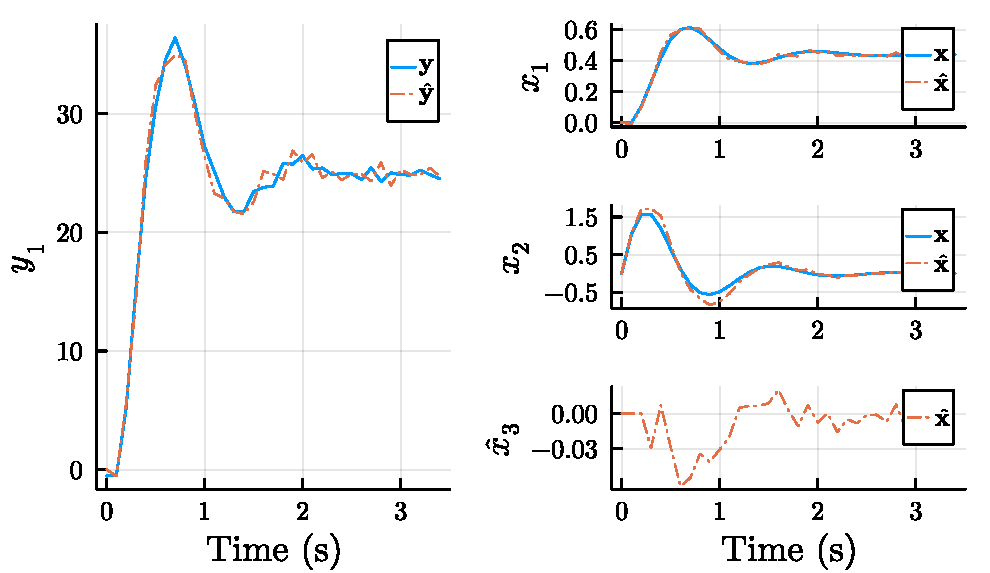
\includegraphics[width=\columnwidth]{fig/plot_NonLinMPC1.pdf}
    \caption{Pendulum state estimation: $y_1 = \theta$ in \si{\degree}, $x_1=\theta$ in \si{\radian}, and $x_2=\omega$ in \si{\radian\per\second}.}
    \label{fig:plot_NonLinMPC1}
\end{figure}

\cref{fig:plot_NonLinMPC1} indicates that the Kalman filter performance seems sufficient for control. The estimate $\hat{x}_3$ is the integrating state on the torque $\tau$ that compensates for static errors. 

\subsubsection{Nonlinear Model Predictive Controller}

As the motor torque is limited to \num{-1.5} to \SI{1.5}{\newton\meter}, the input constraints are incorporated to a \texttt{NonLinMPC} object:
\begin{minted}{julia}
mpc = NonLinMPC(estim, Hp=20, Hc=2, Mwt=[0.5], Nwt=[2.5])
mpc = setconstraint!(mpc, umin=[-1.5], umax=[+1.5])
\end{minted}
\spacerepl
\begin{minted}{julia-repl}
NonLinMPC controller with a sample time Ts = 0.1 s, Ipopt
optimizer, UnscentedKalmanFilter estimator and:
 20 prediction steps Hp
  2 control steps Hc
  1 manipulated inputs u (1 integrating states)
  3 states x̂
  1 measured outputs ym (0 integrating states)
  0 unmeasured outputs yu
  0 measured disturbances d
\end{minted}

The keyword arguments \texttt{Mwt} and \texttt{Nwt} are the output setpoint tracking and move suppression weights, respectively. An angular setpoint of \SI{180}{\degree} (inverted position) test \texttt{mpc} performance on the plant: 

\begin{minted}{julia}
x0 = [0, 0]; x̂0 = [0, 0, 0]
res = sim!(mpc, N, [180]; plant, x0, x̂0)
plot(res)
\end{minted}

\begin{figure}[h]
    \centering
    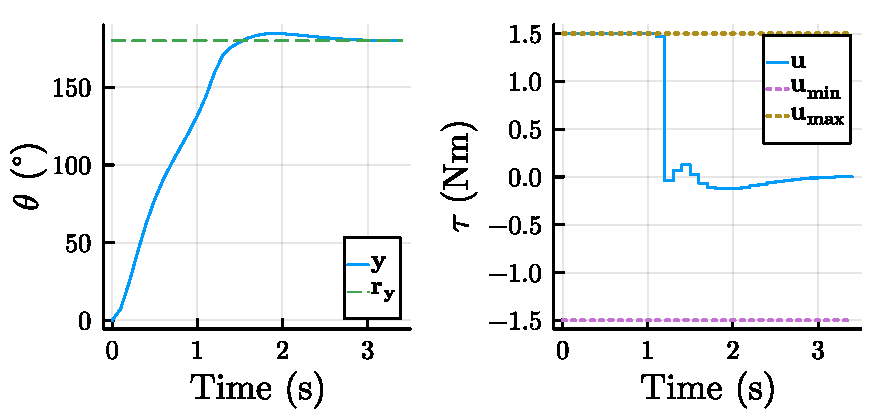
\includegraphics[width=\columnwidth]{fig/plot_NonLinMPC2.pdf}
    \caption{Pendulum output setpoint tracking: $y_1 = \theta$ in \si{\degree} and $u_1 = \tau$ in \si{\newton\meter}.}
    \label{fig:plot_NonLinMPC2}
\end{figure}

The result in \cref{fig:plot_NonLinMPC2} suggests that the controller is robust enough to variations on $K$ coefficient. Starting from this inverted position, the closed-loop response to a step disturbances of \SI{10}{\degree}:

\begin{minted}{julia}
x0 = [π, 0]; x̂0 = [π, 0, 0]
res = sim!(mpc, N, [180.0]; plant, x0, x̂0, y_step=[10])
plot(res)
\end{minted}

\begin{figure}[h]
    \centering
    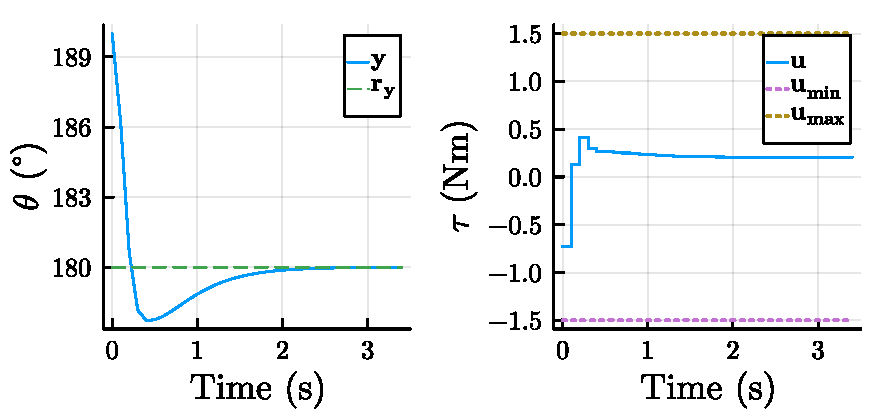
\includegraphics[width=\columnwidth]{fig/plot_NonLinMPC3.pdf}
    \caption{Pendulum load disturbance rejection : $y_1 = \theta$ in \si{\degree} and $u_1 = \tau$ in \si{\newton\meter}.}
    \label{fig:plot_NonLinMPC3}
\end{figure}

is satisfactory, as presented in \cref{fig:plot_NonLinMPC3}.

